\chapter{Conclusion}
\`A l'issue de ces 11 semaines de stage passées dans l'entreprise \mbx{}, je souhaite faire un bilan professionnel, technique mais également personnel de ce que m'a apporté mon travail au sein de l'équipe de développement de \adt{}.

Dans les pages qui suivront cette conclusion, vous pourrez observer mon Curriculum Vitae avant et après le stage afin de mieux observer ma progression. Un bilan de compétences est également disponible.
\section{Bilan professionnel}
    Ce stage fut ma première experience professionnel, cela m'a permis de voir que cela n'avait rien à voir avec le monde universitaire.

    En effet, j'ai découvert qu'en entreprise, nous n'avons pas le droit à l'erreur, je travaillais sur \adt{} qui est actuellement utilisé par des clients, ainsi, mes modifications passait en production, il fallait donc que je test correctement mon travail afin que les clients n'ai pas de problème lors de l'utilisation de l'application.

    \'Egalement, j'ai appris qu'en entreprise, il faut vraiment prévoir tous les cas d'utilisations, qu'un seul cas oublié peut être catastrophique pour le produit.

    Enfin, je me suis rendu compte que dans le monde du travail, les programmes sont loin d'être récents, ainsi le développement de \adt{} ayant été commencé dans les années 2000, j'ai eu du mal à comprendre certaines parties du code, j'ai également découvert du code mort, ce qui ne facilite pas la compréhension du programme. J'ai donc essayé de développer mon application de façon à ce qu'elle soit simple et facile à comprendre, cependant je sais que dans 10 ans, mon code sera vieux, difficile à comprendre et à maintenir.

    Même après mon départ, mon travail sera utilisé et amélioré, cela me fait plaisir, et change de l'IUT où une fois finis on entend plus parler de notre travail. Cependant c'est également plus difficile étant donné qu'il faut développer notre application de façon à ce qu'elle puisse être continuée facilement.
\section{Bilan technique}
D'un point de vue technique, ce stage m'a permis d'apprendre de nouvelles technologies que je ne connaissais pas, Adobe AIR d'une part, je ne connaissais pas son existence, et cela m'a montré qu'avec des technologies web, il est de nos jours possible de faire tout ce que l'on veut.

J'ai aussi appris le JavaScript qui ne nous est pas enseigné à l'IUT, mais également le PHP orienté objet, cependant ma formation en Algorithmique et en technologies web m'a permis de rapidement apprendre ces nouvelles technologies.

Enfin, ce stage m'a également montré que l'optimisation dans le cadre du web est très importante, en effet nous ne savons pas d'avance combien de personnes se connecterons sur le serveur en simultané, ainsi il faut faire attention au moindre octet afin que le serveur n'ai aucun problème, j'ai ainsi appris qu'en informatique la notion d'infini n'existe pas, par exemple, une requête SQL doit toujours avoir une limite afin d'éviter les problèmes.

Cela m'a montré qu'un analyste programmeur n'arrête jamais d'apprendre, toute sa carrière il doit se mettre à niveau, en effet l'évolution de l'informatique étant très rapide, un développeur ne peut se contenter de ses connaissance.

\section{Bilan personnel}
    Sur un plan personnel, ce stage fût une excellente expérience, cela m'a conforté dans mon choix de poursuivre mes études. En effet le stage était très intéressant, cependant je souhaite aller plus loins afin d'avoir accès à des postes de responsable et de pouvoir évoluer tout du long de ma carrière.\\
    J'ai donc choisis d'aller en L3 afin de continuer vers un master.

    Cela m'a également montré que j'étais capable de m'intégrer rapidement dans une équipe de développement, et que je pouvais ainsi poser ma pierre à l'édifice. Ce stage m'a donné confiance en moi, m'a montré que mes connaissances techniques actuelles pouvaient me permettre de développer beaucoup de choses, cependant mon avidité de connaissances me pousse à continuer.

    Afin de continuer à faire évoluer le produit, j'ai eu la chance d'être employé en CDD au mois de juillet dans cette entreprise, cela me permettra je l'espère d'avoir une meilleure vision du future de l'application.

\vfill
\textit{Ci-après mon cv avant et après le stage}.
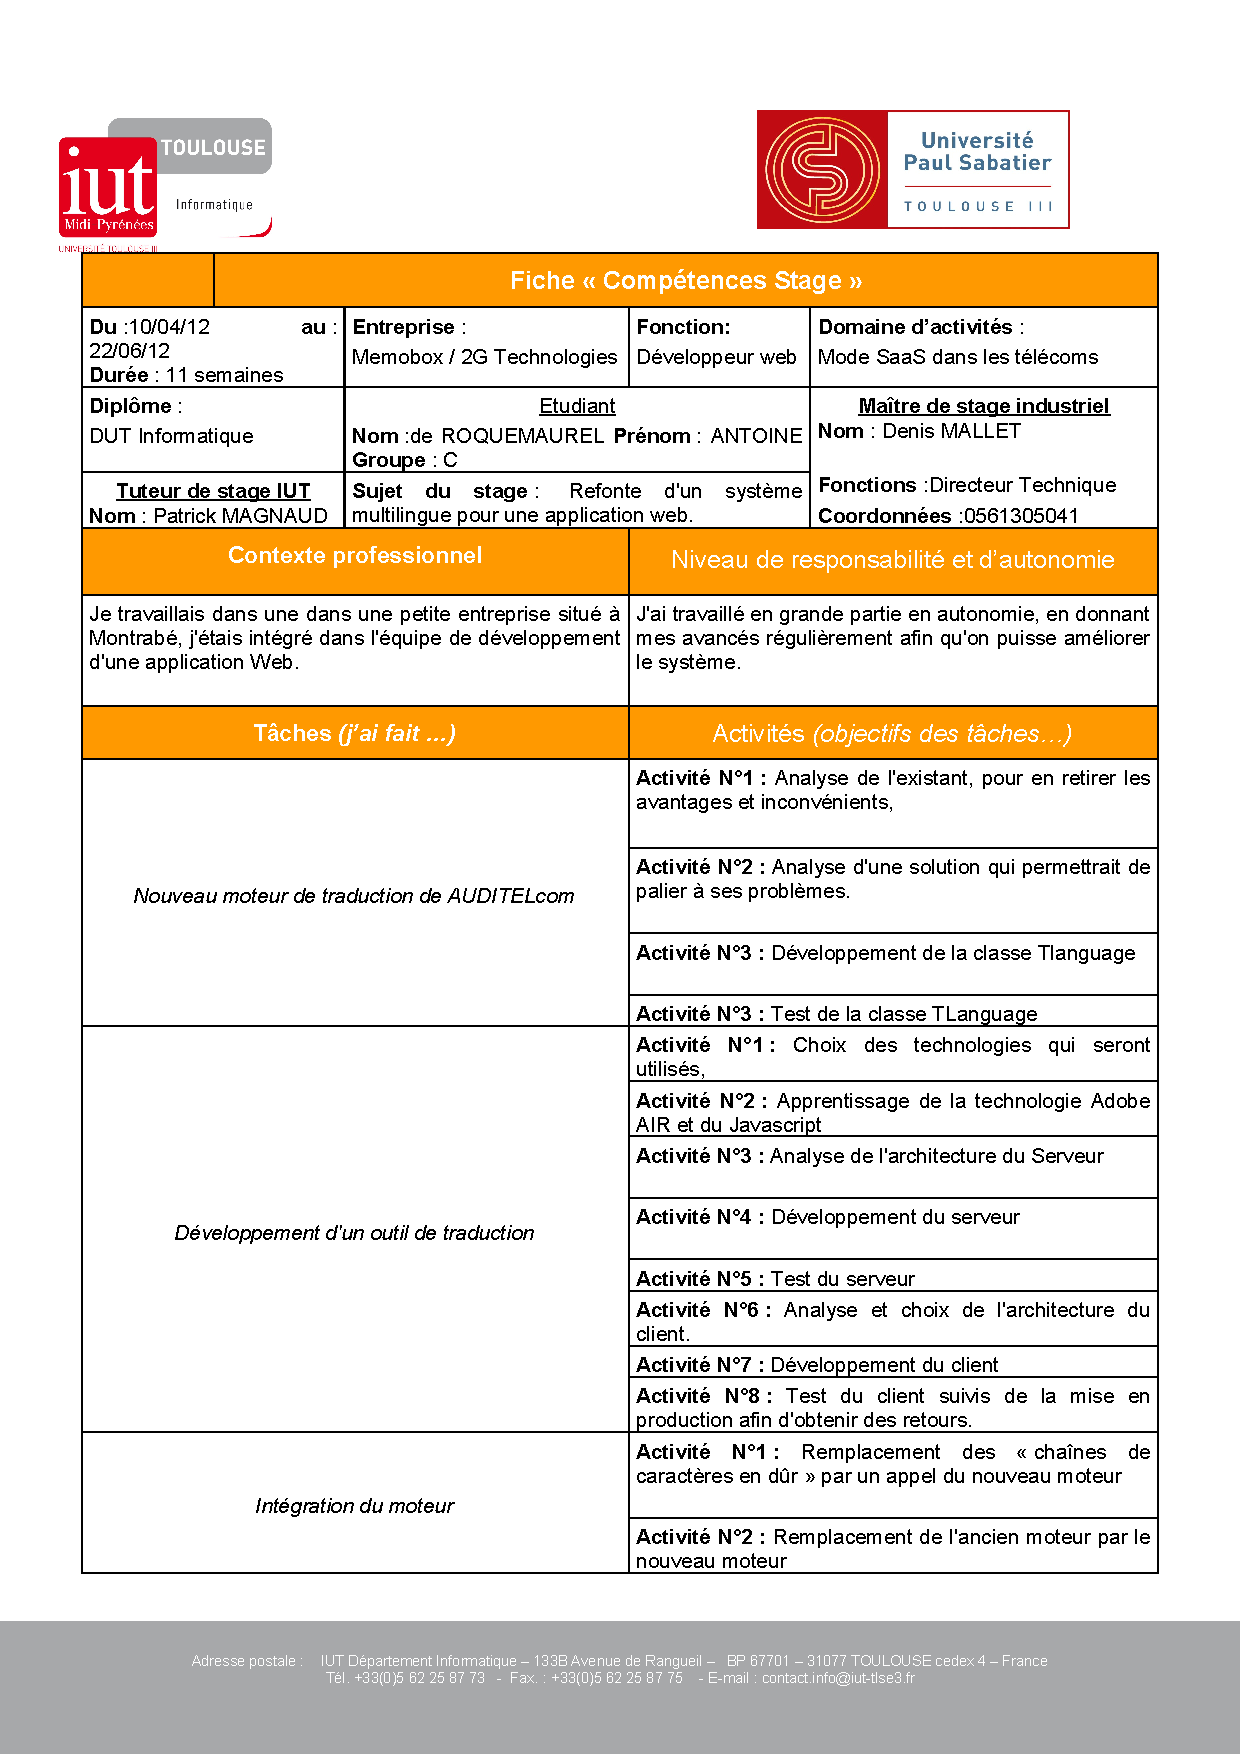
\includepdf[pages=1-3]{competences.pdf}
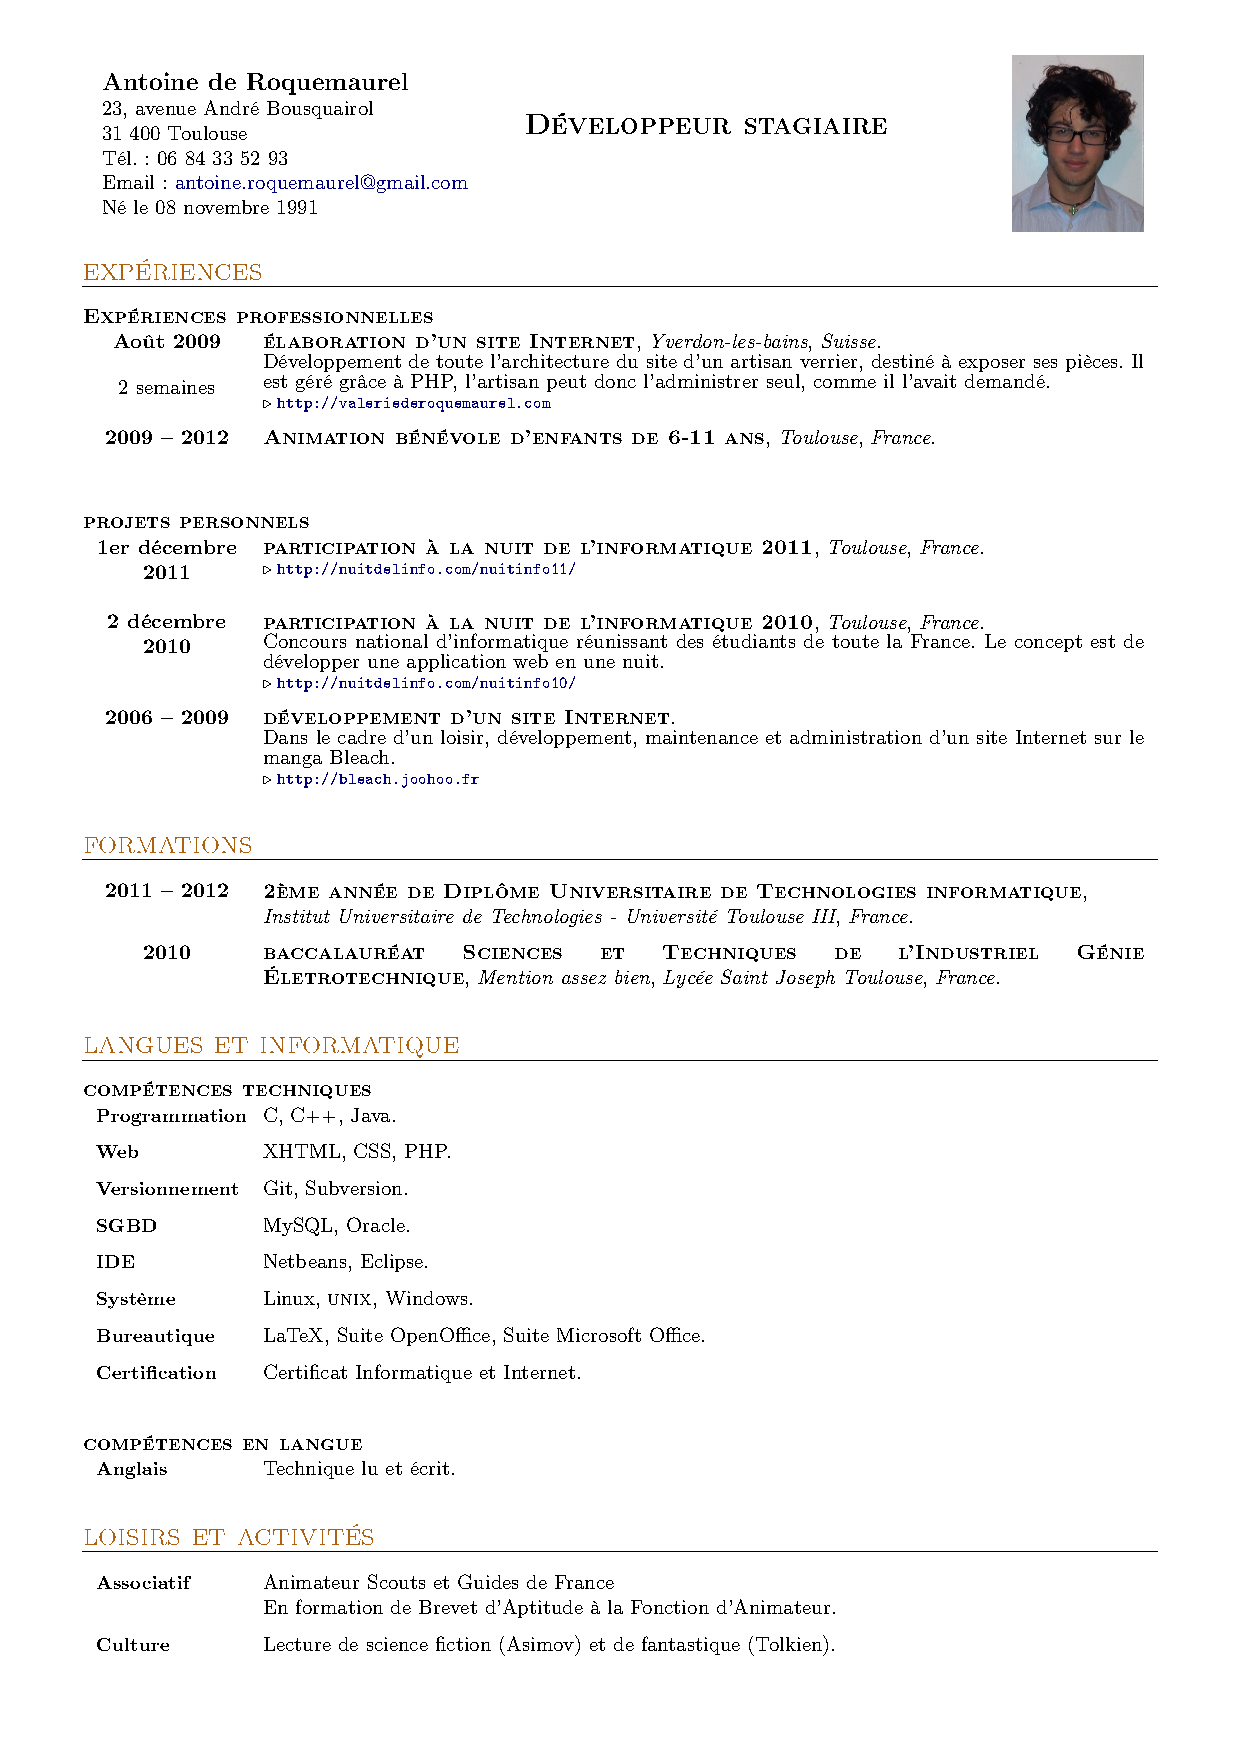
\includepdf{images/oldCV.pdf}
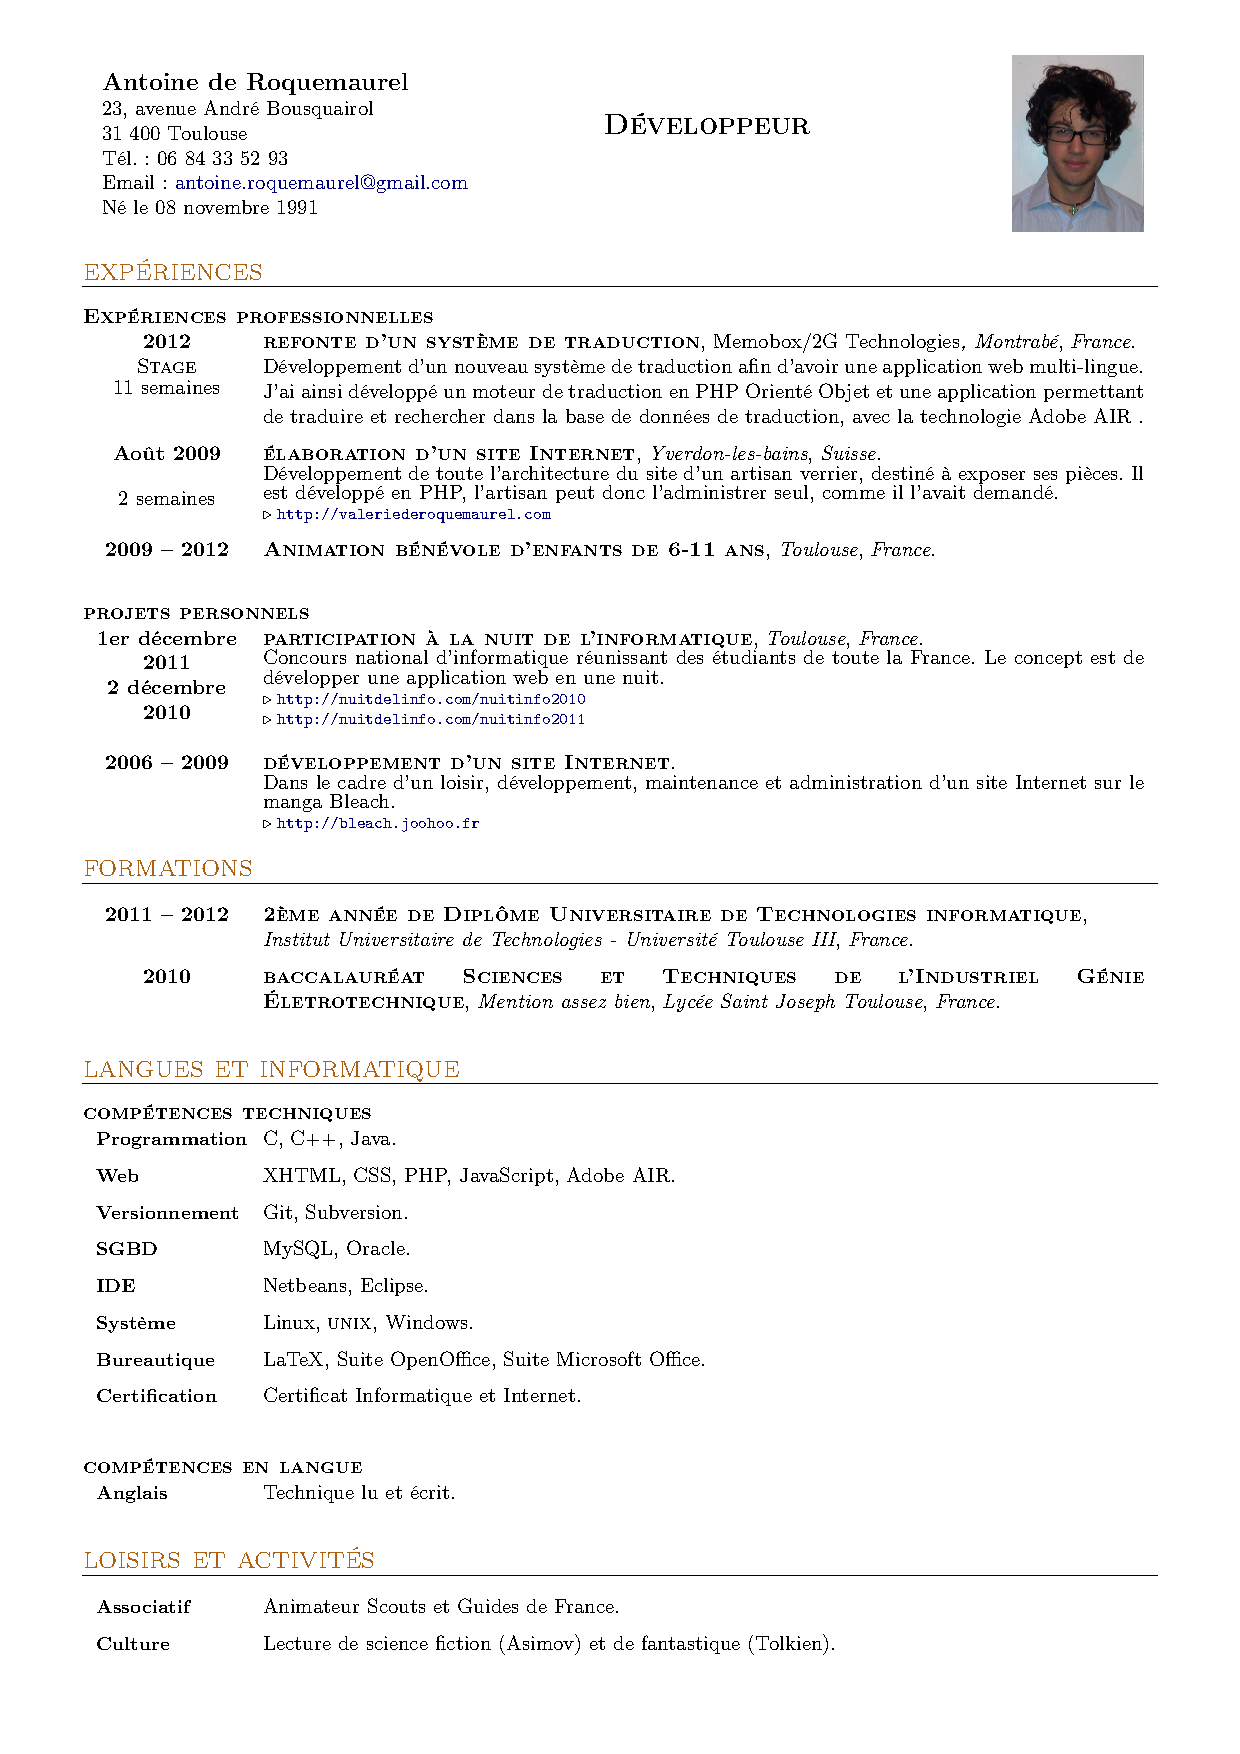
\includepdf{images/newCV.pdf}
